\documentclass[a4paper; 11pt]{article}
\usepackage[utf8]{inputenc}
\usepackage[english]{babel}
\usepackage{graphicx}
\usepackage{multicol}
\usepackage{amsmath}
\makeatletter
\setlength{\@fptop}{0pt}
\makeatother
\setlength{\columnsep}{1cm}
\bibliographystyle{unsrt}
\begin{document}

\title{Usability of Mobile Map Applications}

\author{Rachel Rivera\\
Professor: Dr. Dionisio\\
CMSI 370: Interaction Design\\
  Loyola Marymount University}

\date{September 25, 2014}

% Create title page with no page number

\renewcommand{\thefootnote}{\fnsymbol{footnote}}



%\singlespacing

\maketitle

\vspace{-.2in}
\begin{center}
\begin{abstract}
\noindent This investigation is motivated by the increasing significance of the usability of systems in today's competitive technology market. Usability testing and usability evaluations have become important tools in the assessment of user interfaces. This paper presents empirical mobile usability studies of two distinct map applications: Google Maps and Apple Maps. Participants of this investigation were asked to carry out three tasks with each mobile map application. The results of this examination include (a) the contextual factors studied; (b) quantitative data collected from each task; (c) a brief qualitative review of the applications from each participant; and (d) the core usability metrics measured. This paper not only presents the usability metrics collected by the study but also presents a heuristic evaluation of each map application.
\end{abstract}
\end{center}

\medskip
\medskip


\medskip
\noindent \textit{Group Members}: Katarina Klask, J.B. Morris, Alex Schneider, Khalid Seirafi, and Ronald Uy.

\thispagestyle{empty}

\clearpage

%\onehalfspacing
\setcounter{footnote}{0}
\renewcommand{\thefootnote}{\arabic{footnote}}
\setcounter{page}{1}

\section{Introduction}
When the Apple Maps mobile application was first released as part of iOS 6 in September 2012, it received a significant amount of negative feedback. Walt Mossberg of the \textit{Wall Street Journal} was one of many who thought that Apple Maps was the biggest drawback of the iPhone 5.\cite{Mossberg} At this time, the Google Maps mobile apps, on both iOS and Android, were used by roughly 81 million people.\cite{ComScore} However, Apple Maps grew, matured, and began gaining traction. By September 2013, Apple Maps gained 35 million regular users. The number of users of Google Maps dropped to around 58.7 million at this time.\cite{ComScore} Although the Apple Maps mobile app is newer than the Google Maps mobile app,\footnote{The initial release of Google Maps for Mobile was in September of 2008.} the two map applications are comparable with respect to features they provide as well as popularity nowadays.
\medskip
\par
Since both Google Maps apps and Apple Maps apps are widely known and used, it is important that the usability metrics of the two systems are examined. Thus, this study aims to empirically investigate the usability of each application. The current consensus within the field of interaction design is that usability depends on five distinct metrics: \textit{learnability}, \textit{efficiency}, \textit{errors}, \textit{memorability}, and \textit{satisfaction}.\cite{Nielsen} The three metrics on which this particular study focuses are efficiency, errors, and satisfaction.
\section{Contextual Factors}
Prior to having each test subject perform the tasks, a little contextual data about the users was first collected. Users were asked about their previous experience with Apple Maps as well as their previous experience with Google Maps.
\vspace{-.2in}
\begin{figure}[ht]
\begin{center}
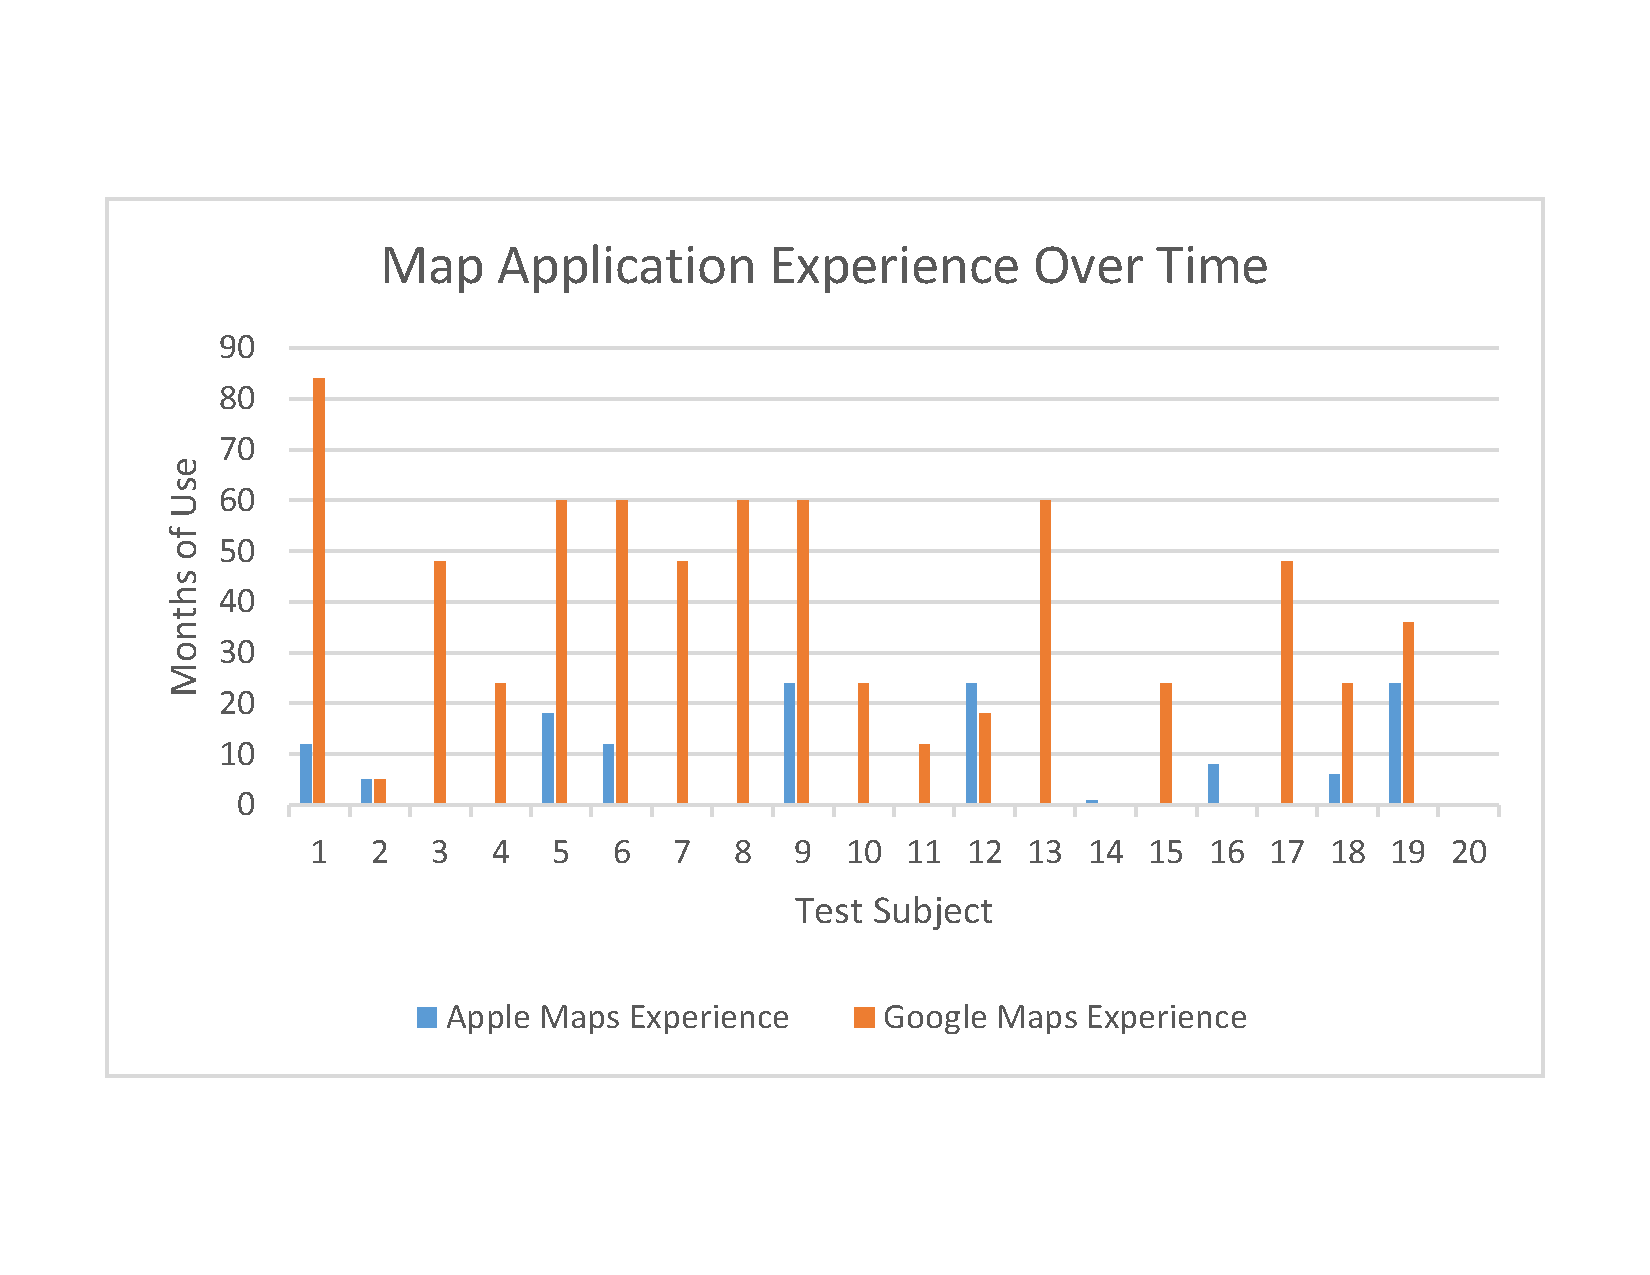
\includegraphics[keepaspectratio, width=.7\textwidth ]{user_context.pdf}
\end{center}
\end{figure}
\clearpage
\par
The fact that nearly every test subject had significantly more Google Maps experience than Apple Maps experience was a challenge in the conducting of this study.  Since this study aimed to test the usability metric of efficiency, and \textit{not} that of learnability, we did not test subjects if they had no prior experience with the application. For future studies, however, it might be worthwhile to give inexperienced users a short tutorial so it is possible to test them thereafter.



\section{The Experiment} \label{sec:Experiment}
Each person who participated in this study had to carry out three concrete tasks with the map application[s] with which they were experienced.
\begin{enumerate}
  \item Save a pin anywhere on the map and get driving directions to that pin.
  \item Find the location of the nearest Vons.
  \item Find the fastest route from the current location to LACMA.
\end{enumerate}
In order to keep the study as controlled as possible, all testing was done on iOS devices (no map applications of android devices were tested). As test subjects executed the tasks, information was collected pertaining to their efficiency, errors, and satisfaction.


\section{Usability Metrics}
\subsection{Efficiency}
\par
\textbf{First Task: }Drop a pin on the map and get driving directions to that pin.
\vspace{-.4in}
\begin{figure}[ht]
\begin{center}
\vspace{-.1in}
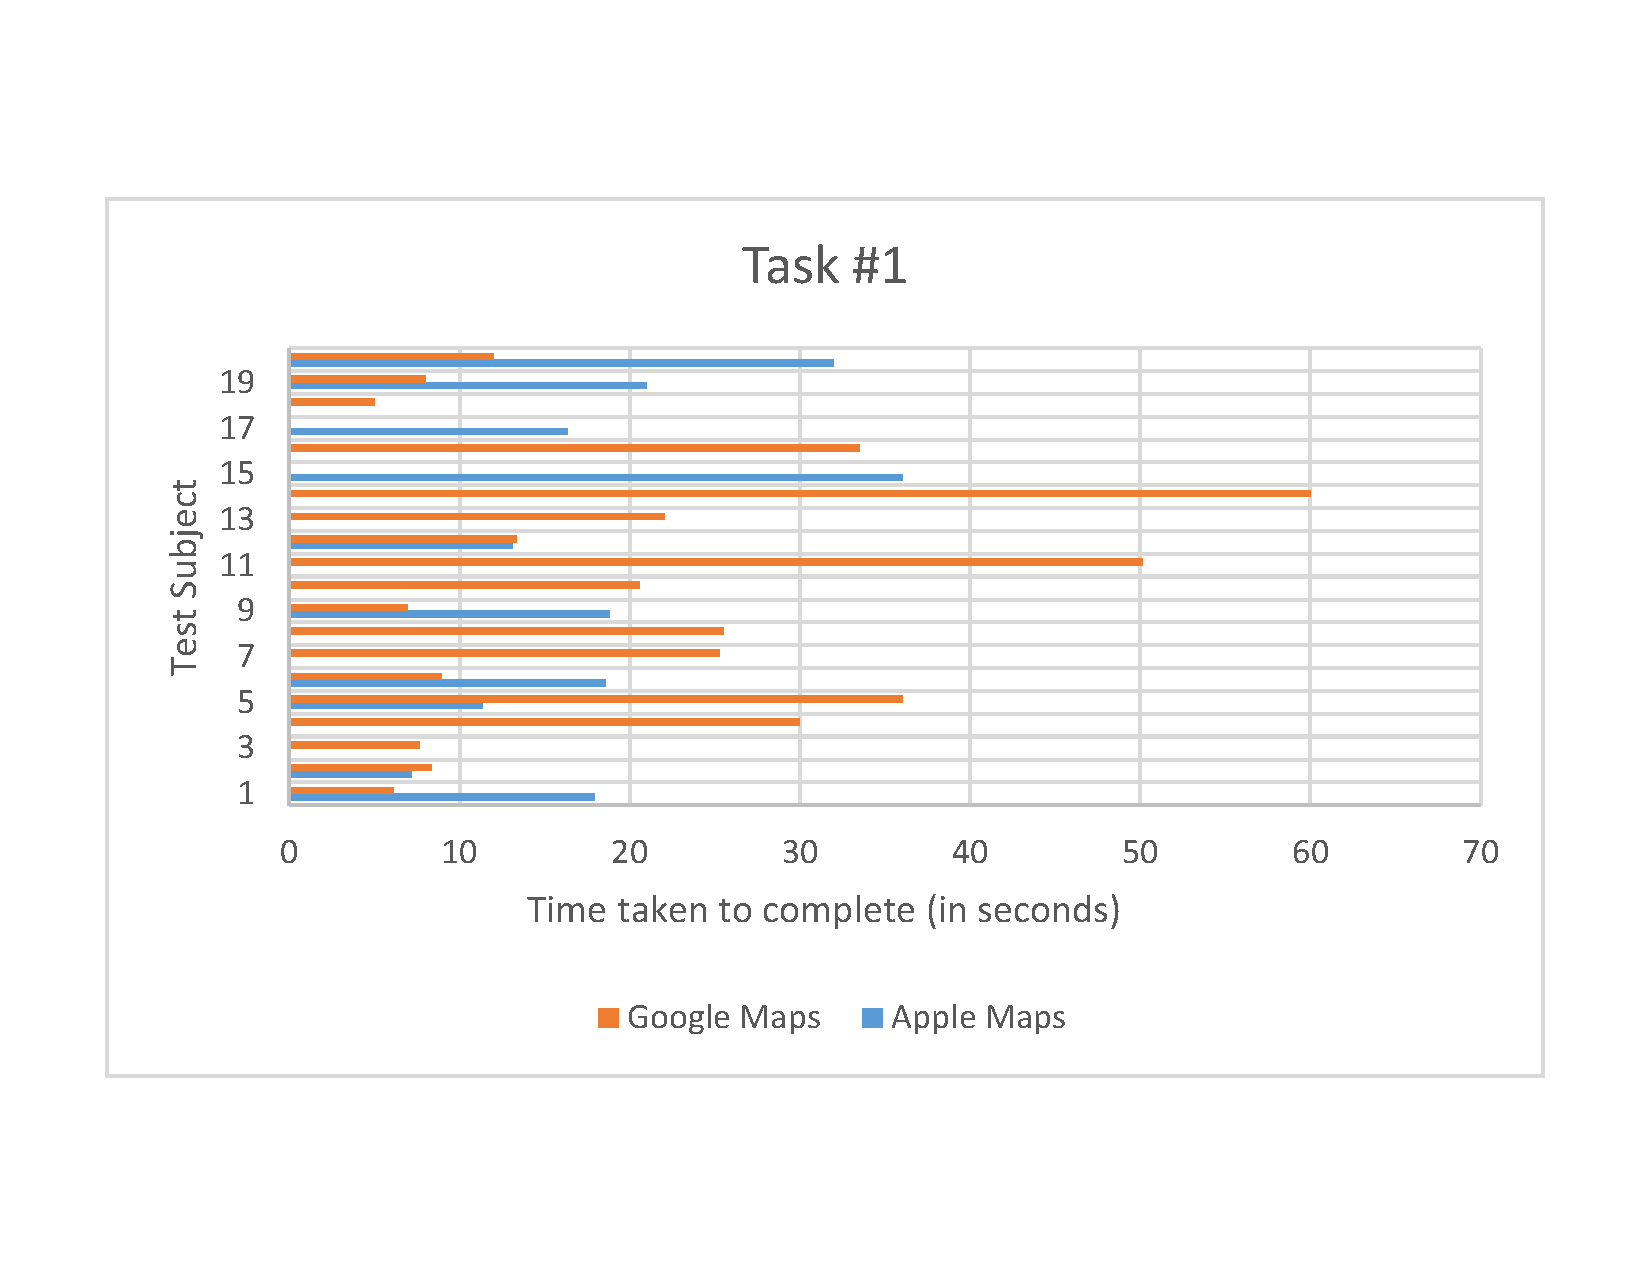
\includegraphics[keepaspectratio, width=.8\textwidth ]{task1.pdf}
\end{center}
\end{figure}
\begin{center}
\vspace{-.6in}
\par
Average time for task \#1 on Google Maps app: $ \approx $ \textit{21.08 seconds}
\par
Average time for task \#1 on Apple Maps app: $ \approx $ \textit{19.24 seconds}
\end{center}
\par
\noindent
This task's results suggest that users are more efficient using Apple Maps. \footnote{Though subjects using Apple Maps were more efficient \textit{on average}, it notable that there were a couple of anomalies within the Google Maps users who significantly raised the average.}
\medskip
\medskip
\par
\noindent
\textbf{Second Task: }Find the location of the nearest Vons.
\begin{figure}[ht]
\begin{center}
\vspace{-.5in}
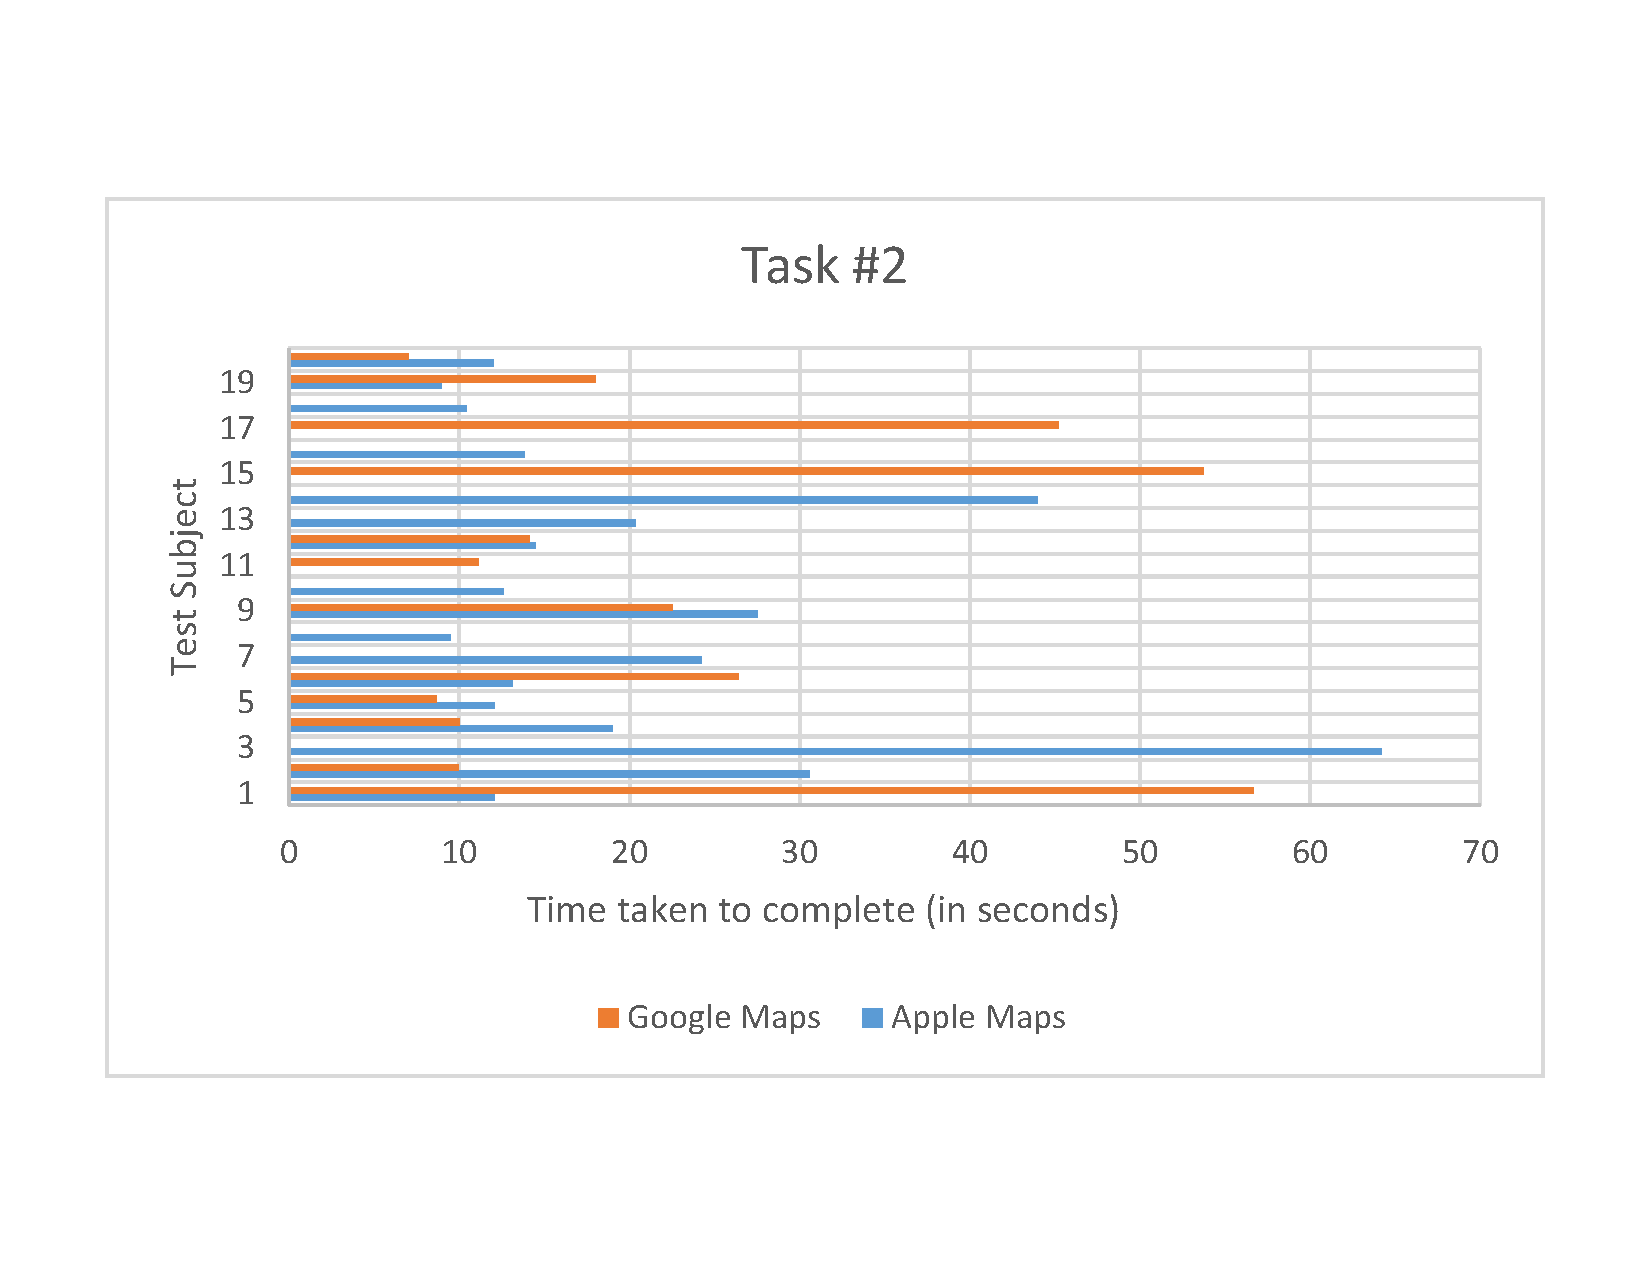
\includegraphics[keepaspectratio, width=.8\textwidth ]{task2.pdf}
\end{center}
\end{figure}
\begin{center}
\vspace{-.6in}
\par
Average time for task \#2 on Google Maps app: $ \approx $ \textit{20.53 seconds}
\par
Average time for task \#2 on Apple Maps app: $ \approx $ \textit{23.62 seconds}
\end{center}
\par
\noindent
This task's results suggest that users are more efficient using Google Maps. 
\medskip
\medskip
\par
\noindent
\textbf{Third Task: }Find the fastest route from the current location to LACMA.
\begin{figure}[ht]
\begin{center}
\vspace{-.4in}
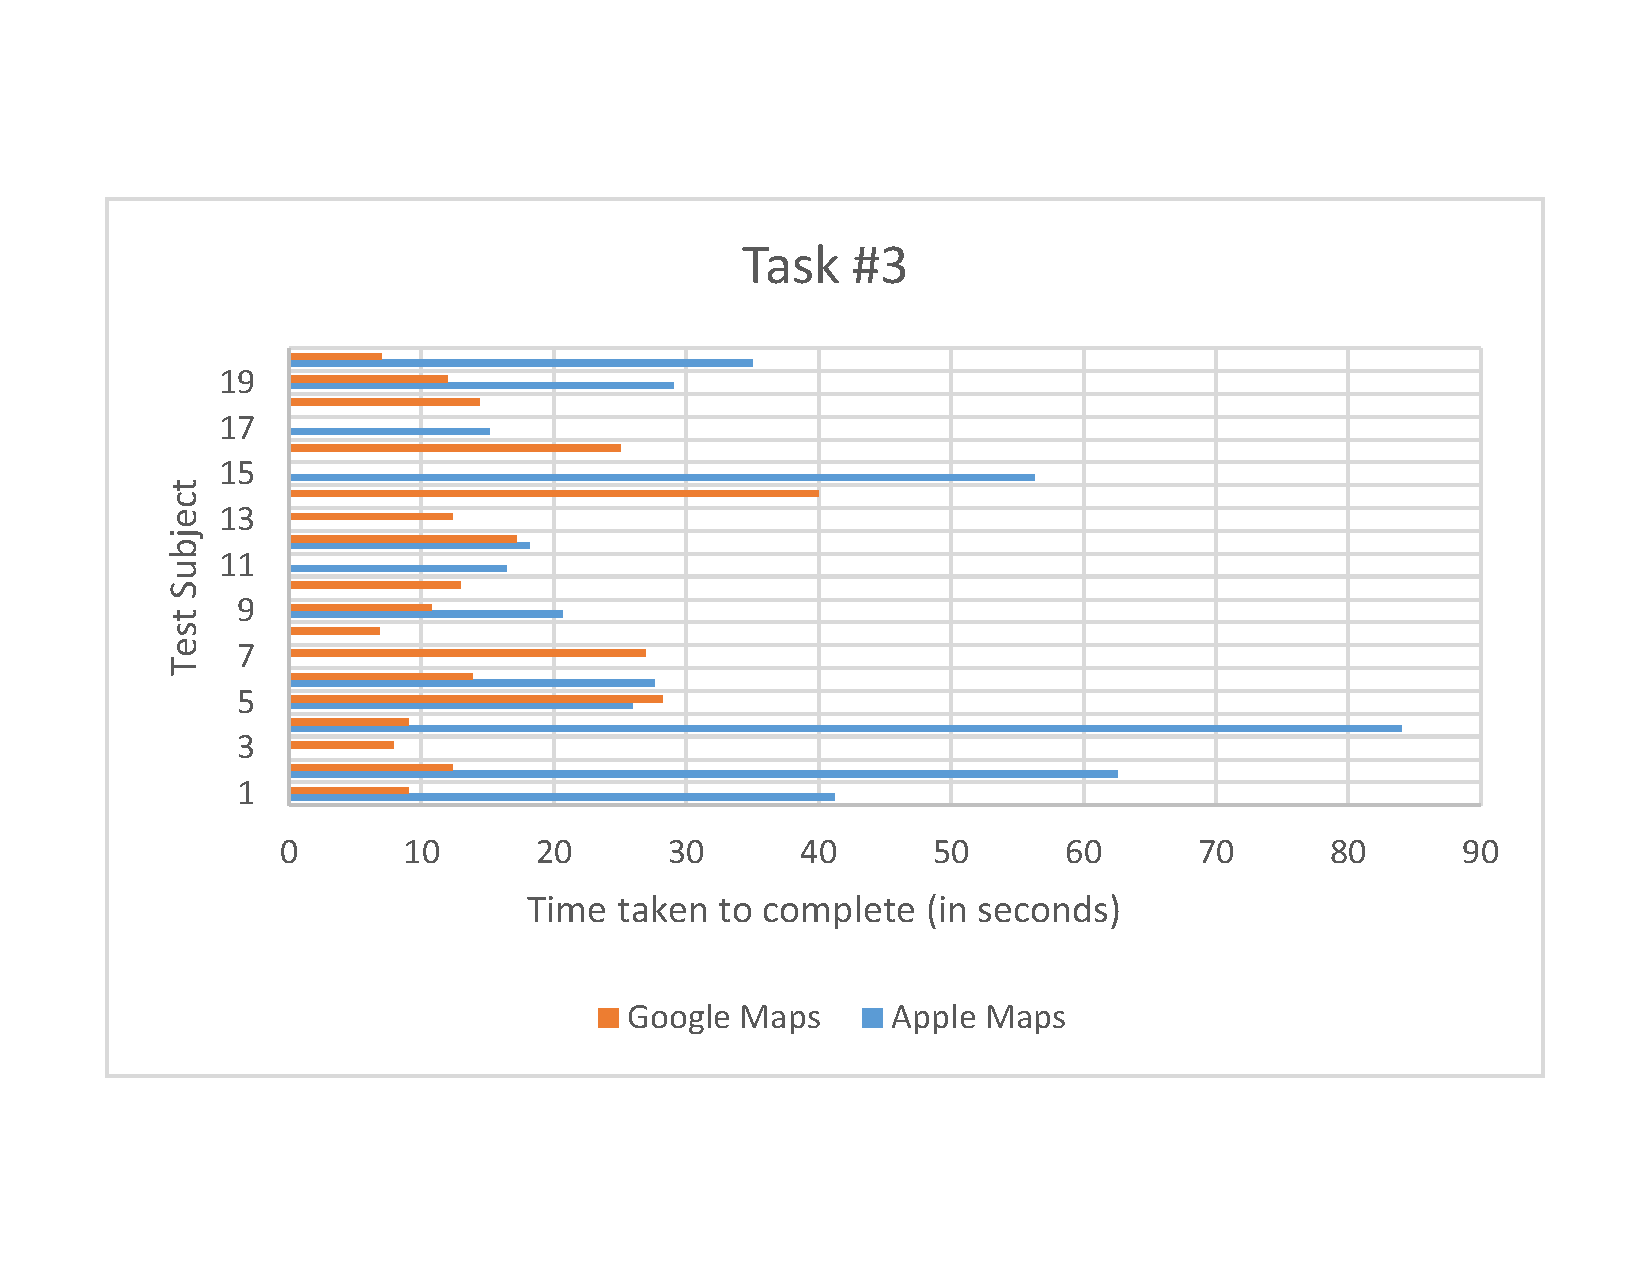
\includegraphics[keepaspectratio, width=.8\textwidth ]{task3.pdf}
\end{center}
\end{figure}
\begin{center}
\vspace{-.4in}
\par
Average time for task \#3 on Google Maps app: $ \approx $ \textit{15.62 seconds}
\par
Average time for task \#3 on Apple Maps app: $ \approx $ \textit{35.98 seconds}
\end{center}
\par
\noindent
This task's results suggest that users are more efficient using Google Maps. 

\subsection{Errors}
\par
The only errors collected by this study were incidents wherein the user did something whose result is not what he or she anticipated. The table on the following page shows you some examples of errors from this investigation.

\begin{table}[ht]
\centering
\begin{tabular}{l|c|c}
Task & Application & Specific Error\\\hline
Task1 & Apple Maps & hit `Share' button to try to map to pin \\
Task1 & Google Maps & hit `Near You' button to try to drop pin\\
Task2 & Apple Maps & tried to manually search for ``Nearest Vons"\\
Task2 & Google Maps & voice command attempt instead of search\\
Task3 & Apple Maps & hit `Current Location' for directions\\
Task3 & Google Maps & found side streets when expecting highway route
\end{tabular}
\end{table}
\par
The percentage of subjects with errors is analyzed rather than solely the numbers of errors since more subjects tested the Google Maps app than Apple Maps app.
\begin{table}[ht]
\begin{tabular}{l c c c c}
& \multicolumn{4}{c}{}\\ % Amalgamating several columns into one cell is done using the \multicolumn command as seen on this line
& \textbf{Task1} & \textbf{Task2} & \textbf{Task3} \\
Percentage of Apple Users with Errors & \textit{40\%} & \textit{50\%}  & \textit{20\%} \\
Percentage of Google Users with Errors & \textit{29.4\%} & \textit{17.6\%}  & \textit{11.7\%} \\

\end{tabular}

\end{table}
\par
The results suggest that Google Maps is more usable with respect to errors.

\subsection{Satisfaction}
\begin{figure}[ht]
\begin{center}
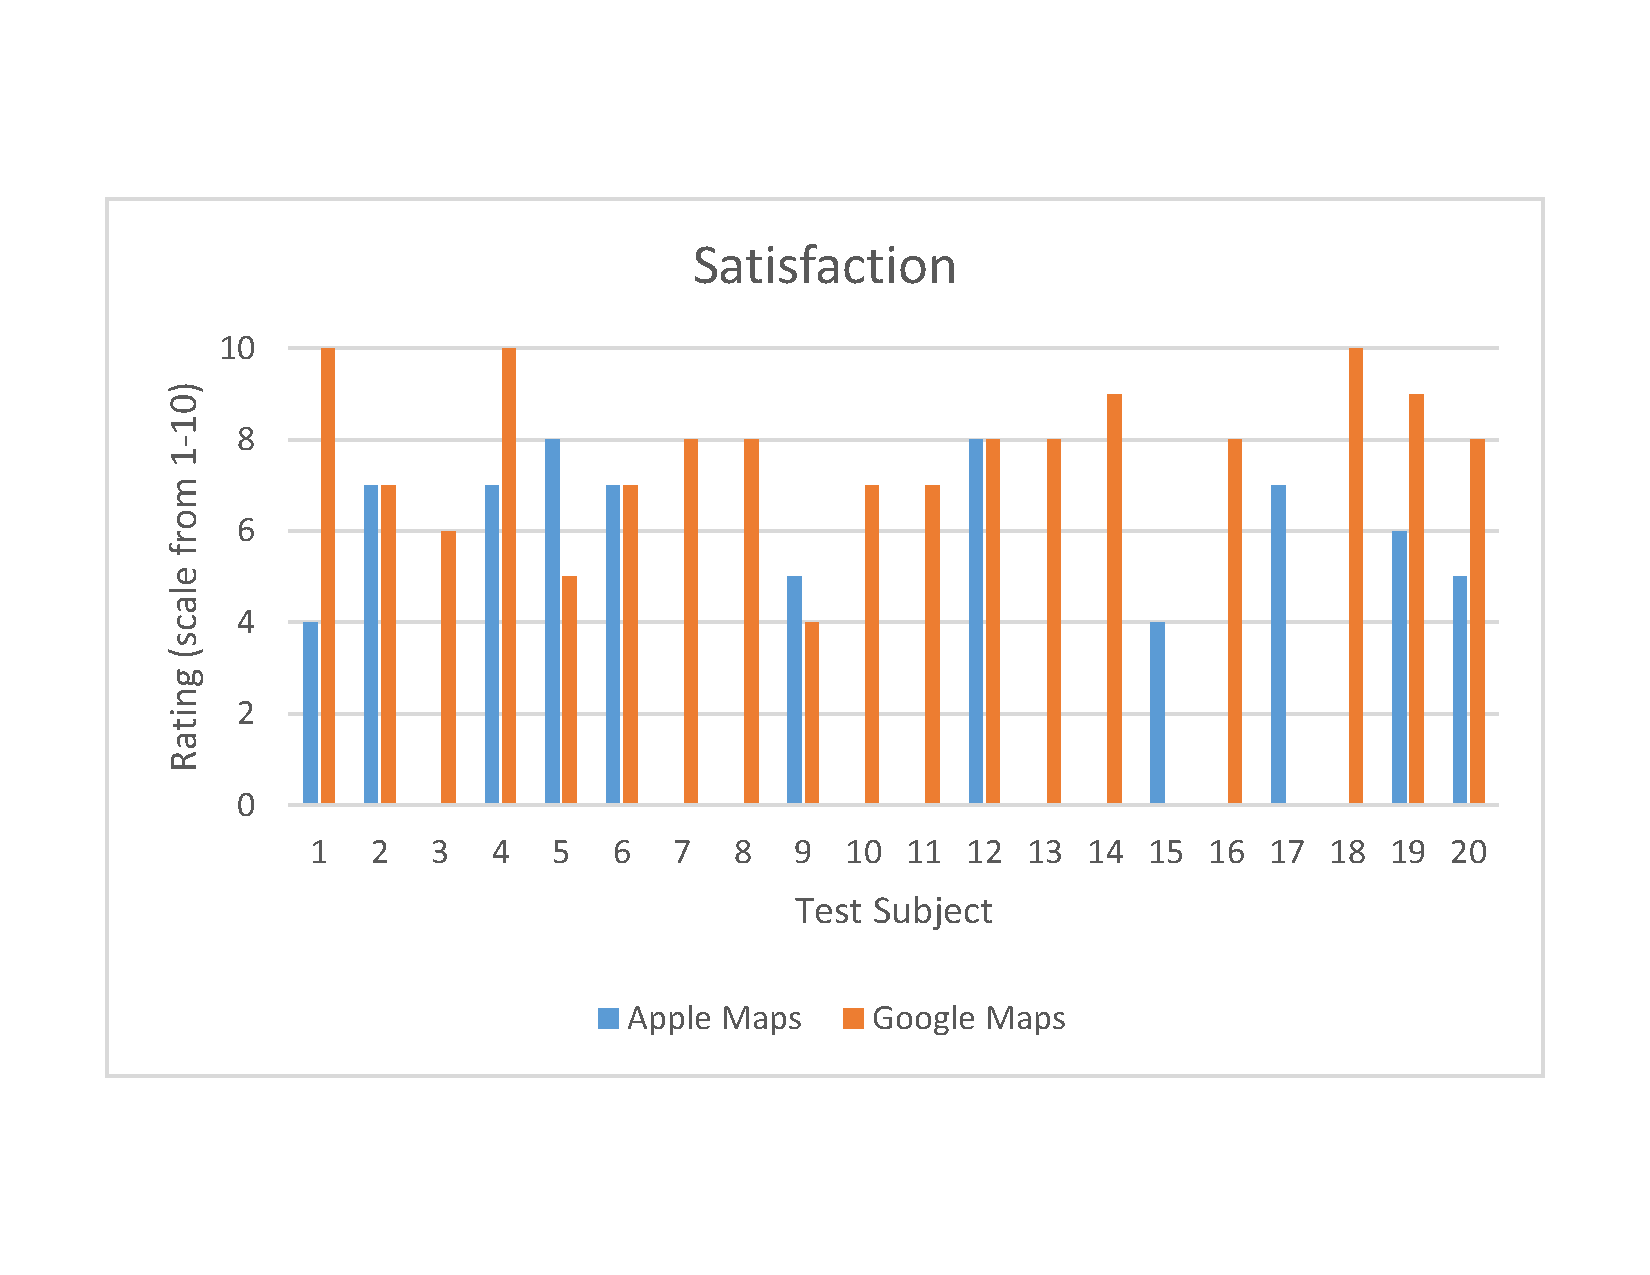
\includegraphics[keepaspectratio, width=.8\textwidth ]{satisfaction.pdf}
\end{center}
\end{figure}
\par
Satisfaction ratings were on a scale from 1 to 10.
\par
Average rating for Apple Maps: $ \approx $ \textit{6.18}
\par
Average rating for Google Maps: $ \approx $ \textit{7.72}

\begin{multicols}{2}
[
\section{Heuristic Evaluation}
Though usability metrics are extremely important in assessing a system, it is also important to heuristically evaluate systems in order to explore \textit{why} they performed the way they do.
My heuristic evaluations of the mobile map applications will be based on the guidelines documents that correspond to the applications.
\subsection{Google Maps}
]
The icons of the Google Maps mobile application comply with the Google Design Guidelines\cite{Google}: simple, modern, and geometric in execution. However, Google Maps completely fails to use any standard iOS icons\cite{Apple}:
\par
\noindent

\includegraphics[width=.45\textwidth]{ios-bar-icons.png}
\par
\noindent
Though it is not required to use these provided iOS icons, the iOS HIG (Human Interface Guidelines) state that it is ``a good idea to use the built-in icons as much as possible because users already know what they mean."\cite{Apple} Balancing consistency in platform with consistency of brand is a challenge, but there is a possibility that adhering more to the iOS HIG could improve usability of Google Maps even more. There was a higher percentage of errors specifically involving clicking wrong icons in the Google Maps application than there was in the Apple Maps application. 

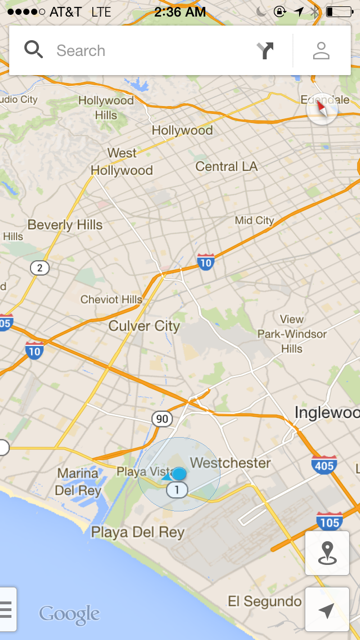
\includegraphics[width=.5\textwidth]{google-maps.png}


\end{multicols}
\clearpage
\begin{multicols}{2}
[
\subsection{Apple Maps}
]
\par
\noindent
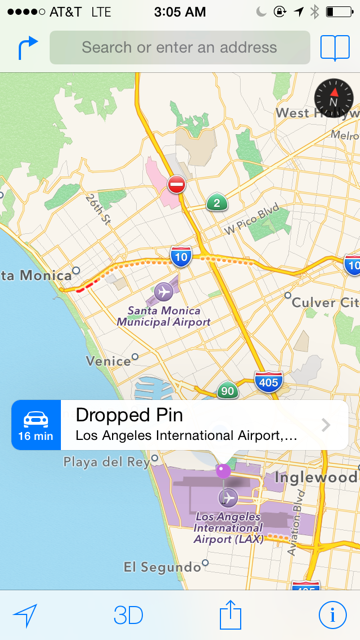
\includegraphics[width=.5\textwidth]{apple-maps.png}
\par
\noindent
One guideline from iOS HIG is that important content or functionality should be `elevated':\cite{Apple}
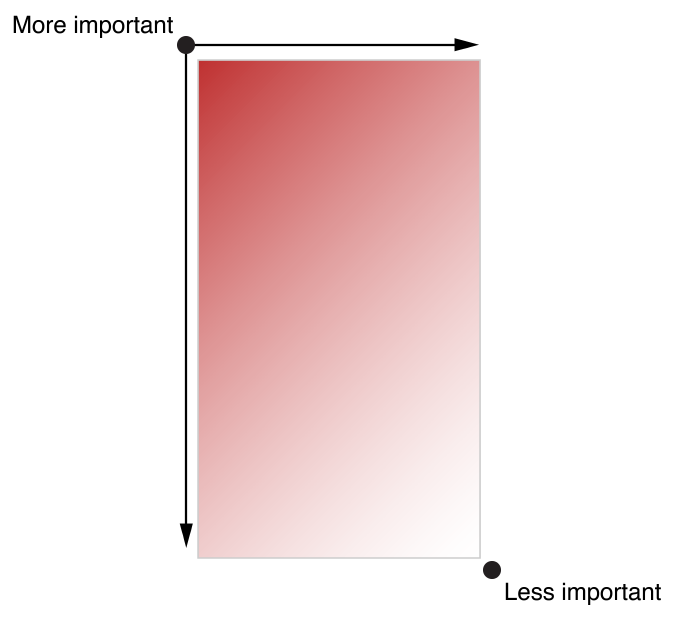
\includegraphics[width=.35\textwidth]{apple-importance.png}
\par
\noindent
This suggests that the icon on the top left-hand corner, which takes you to the directions screen in this case, is the most important. I would have to agree that getting directions is very important functionality, so it seems as if the app is complying to the guidelines. However, a couple of test subjects tried to click on the icon second from the right on the bottom for directions. It is possible that this guideline of important functionality being `elevated' may not be intuitive to all users.
\end{multicols}
\medskip
\medskip
\par
The lack of standard iOS icons in the Google Maps app may or may not explain some of the efficiency issues as well as some errors that occurred with the tasks on the mobile Google Maps app. The guideline of important functionality being towards the upper-left corner of the screen may or may not explain some of the efficiency issues as well as errors that occurred with the tasks on the mobile Apple Maps app.
\clearpage
\section{Conclusion}
The usability metrics of the Google Maps mobile application outranked those of the Apple Maps application in almost every way. Though there are some problems with the UI consistency, it does not seem to bother the users (refer back to satisfaction). Still, using non-standard icons or processes isn't without drawbacks. It's loud. It's authorial voice. It's greater cognitive load for users. Anything inconsistent, first or third party is. On an integrated platform like iOS, integrating with the platform offers a lot of benefits, especially when it comes to user experience.

If you use Google apps, either a lot or a little, does the lack of iOS-style buttons make any difference to you?

must recognize that there are limitations to our studies-- didn't test all five metrics; less data for Apple maps; Apple maps is newer; etc.
Judgment call -- google maps with data that we have now.
\clearpage
\begin{thebibliography}{100} % 100 is a random guess of the total number of 
%references
\bibitem{Nielsen} Nielsen, Jakob, \emph{Usability Engineering}, Boston: Academic, 1993.
\bibitem{Mossberg} Mossberg, Walt., ``The iPhone Takes to the Big Screen," \emph{The Wall Street Journal}, September 2012.
\bibitem{ComScore}``Analytics for a Digital World - ComScore, Inc." \emph{ComScore, Inc}, 2012.
\bibitem{Google} \emph{Material Design}, www.google.com/design/spec/material-design.
\bibitem{Apple} \emph{iOS Human Interface Guidelines}, https://developer.apple.com/
\end{thebibliography}
%%%%%%%%%%%%% end %%%%%%%%%%%%%%%%%%%%%%%%%%%%%%%



\end{document}